\chapter{\label{ch7-performance}Camera Performance} 

\minitoc

\section{Introduction}

As discussed in Chapter~\ref{ch3-architecture}, it is important that the \gls{chec} camera meets certain criteria in order for it to be accepted as an in-kind contribution to \gls{cta}. One important subset of the criteria is the camera's performance. The requirements that must be fulfilled are driven by the science goal of \gls{cta}. If a camera does not meet the requirements laid out by the \gls{cta} observatory, then it will be refused as a contribution in its current state, lest the science goals of \gls{cta} are not achieved.

This chapter will cover many of the primary standards used to assess a \gls{cta} camera's performance. The results shown in this chapter are all my own, and are obtained using the procedures defined in the preceding chapters. Two important aspects of the camera's performance which are not included in this chapter are the trigger efficiency and absolute photon detection efficiency. The investigations into these parameters are ongoing, of which I have not had direct involvement with as part of my DPhil.

\section{CHEC-S Monte Carlo Model}

An important preface to reporting on the performance of \gls{chec} is the description of the efforts in generating an accurate model of the camera for use inside the Monte Carlo simulations performed by \pkg{sim\_telarray} (Chapter~\ref{ch4-software}). These simulations allow us to more widely explore the parameter space related to our camera performance, and identify potential issues that cause the real camera to drift away from ideal operation. It is also a necessary step in investigating the on-sky performance of the telescope, as:

\begin{itemize}
\item One does not have prior knowledge of the properties of the light incident on the pixels in the real world.
\item The camera is still being tested in the lab. An on-sky campaign for \gls{chec-s} on the \gls{astri} telescope structure is planned for later this year.
\end{itemize}

Contained within the lab data are the parameters required for the Monte Carlo validation process. Important parameters include:

\begin{itemize}
\item Pixel position on the focal surface,
\item Pulse shape for a single photoelectron,
\item Trigger discrimination behaviour,
\item Quantum efficiency (or \gls{pde}),
\item Variation of quantum efficiency between pixels
\item Electronic baseline variation,
\item Photosensor gain,
\item Variation of gain between pixels,
\item \gls{spe} spectrum shape.
\end{itemize}

\begin{figure}
	\centering
    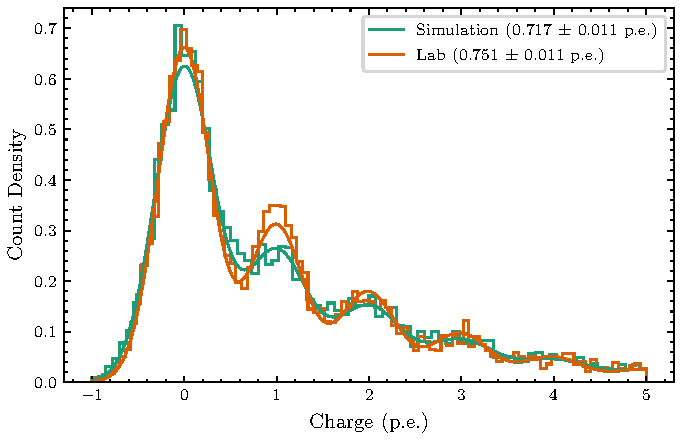
\includegraphics[width=\textwidth]{spe_sim_lab} 
	\caption[Comparison of the SPE spectra between lab measurements and simulations.]{Comparison of the SPE spectra for a single pixel between lab measurements and simulations after an initial attempt towards a more accurate Monte Carlo model. The SPE spectra are identically extracted in both cases, using the \textit{Cross Correlation} charge extraction method. Both spectra are normalised in the x direction by their respective single-photoelectron value, and in the y direction such that their integral is 1.}
	\label{fig:spe_sim_lab}
\end{figure}

\begin{table}[h!]
\centering
\begin{tabular}{ll|ll} \toprule
    Fit Parameter        &            & Simulation          & Lab                \\ \midrule
    Average Illumination & [\si{\pe}] & 0.717 $\pm$ 0.011  & 0.751 $\pm$ 0.011 \\
    Pedestal Deviation   & [\si{\pe}] & 0.314 $\pm$ 0.003  & 0.286 $\pm$ 0.002 \\
    Gain Deviation       & [\si{\pe}] & 0.109 $\pm$ 0.009  & 0.078 $\pm$ 0.007 \\
    Optical Crosstalk    &            & 0.387 $\pm$ 0.007  & 0.350 $\pm$ 0.006 \\ \bottomrule
\end{tabular}
\caption{Parameter values resulting from the fit to the spectra in Figure~\ref{fig:spe_sim_lab}. The \si{1}{$\sigma$} parabolic errors obtained from the covariance matrix of the fit parameters are quoted.}
\label{table:spe_sim_lab}
\end{table}

For the simulation results presented in this thesis, an updated value was obtained for as many of the relevant \pkg{sim\_telarray} parameters as possible. Figure~\ref{fig:spe_sim_lab} displays the resulting differences in terms of the \gls{spe} spectra between lab and simulation. The discrepancies in parameters resulting from the fits to the \gls{spe} spectra are shown in Table~\ref{table:spe_sim_lab}, and are deemed to be close enough for the investigations in this thesis. Further details about the fit procedure for \gls{spe} spectra can be found in Appendix~\ref{a1-spe}. The differences between lab and simulation in other factors and at higher amplitudes are explored through \textit{Charge Resolution} comparisons, investigated later in this chapter.

\section{CHEC-S Charge Resolution}

The \textit{Charge Resolution} is the principle criterion used within \gls{cta} to express how well the camera can resolve a signal. The concept of \textit{Charge Resolution} is introduced in Section~\ref{section:cr}, alongside the \gls{cta} requirement \requirementref{B-TEL-1010 Charge Resolution}. It not only measures the quality of the camera's photosensor and electronics, but also the aptitude of the calibration and signal extraction. Consequently, obtaining a \textit{Charge Resolution} of the camera that meets this requirement has been the underlying driver behind my efforts in developing the techniques described in this thesis.

\subsection{Procedure and Datasets} \label{section:crprocedure}

As directed in the \requirementref{B-TEL-1010 Charge Resolution} requirement, one must validate \textit{Charge Resolution} results in three ways. To achieve this, and understand the relationship between the three validation approaches, four procedures are used to obtain a \textit{Charge Resolution}. The procedures, and their associated name for the purpose of this thesis, are:

\begin{description}
\item [Lab] Utilises uniform illumination datasets taken in the lab that cover the full dynamic range of the camera, with 1000 events at each illumination. The average expected charge per pixel (in photoelectrons) for each illumination is calibrated by the procedure detailed in Section~\ref{section:lab-calib}. Using the calibration procedures detailed in Chapter~\ref{ch5-calibration} and the \textit{Cross Correlation} charge extraction technique (Chapter~\ref{ch6-reduction}), a value of measured charge in photoelectrons is obtained for every waveform. As the average expected charge includes the Poisson fluctuations, it is appropriate to use Equation~\ref{eq:charge_res} for calculating the \textit{Charge Resolution}, with the measured charge per waveform used for ${Q_M}_i$ and the average expected charge for $Q_T$. It is important to note that these datasets are taken with no \gls{nsb} contribution, and are therefore not a completely appropriate measure against the \gls{cta} requirement (defined for an \gls{nsb} photon rate per pixel of $\SI{0.125}{\pe/ns} = \SI{125}{MHz}$). However, a \gls{dcr} of \SI{\sim5}{MHz} is assumed to be present in the \gls{sipmt}.
\item [MCLab] Simulations of the dynamic range datasets from the lab are obtained with the updated \pkg{sim\_telarray} camera model. Using the identical method used for the lab data (excluding the \gls{target} calibration) the charge is extracted and calibrated from the waveforms. The average expected charge for each illumination per pixel is also obtained in the same way as the previous procedure. However, the simulations contain perfect laser uniformity across the camera face (the geometry shown in Figure~\ref{fig:laser_geometry} is still applicable). This dataset then fully represents the same measurements, but with the Monte Carlo model of the camera instead of the physical camera. With an accurate model of the camera, the \textit{Charge Resolution} result should be the same as from the lab measurements. Equation~\ref{eq:charge_res} is also used in this procedure for calculating the \textit{Charge Resolution}.
\item [MCLabTrue] Using the same dataset as the previous procedure, but instead of using the average expected charge, the true number of photoelectrons that were incident on the pixel for each waveform are extracted from the simulation file. The linear fit between the average measured charge and the ``true charge'' is used to calibrate the extracted charge into corresponding units. As the unique value of ``true charge'' per waveform is now used as $Q_T$, Equation~\ref{eq:charge_res2} must be used to account for the lack of Poisson fluctuations in $Q_T$. The \textit{Charge Resolution} resulting from this procedure demonstrates the change in transitioning from ``average expected charge'' to ``true charge'', which is important for interpreting the results from the next procedure.
\item [MCOnsky] A dataset containing Monte Carlo simulations of gamma-ray-induced air shower observations is created using \pkg{CORSIKA} and \pkg{sim\_telarray}. A model of \gls{chec-s} on the \gls{astri} telescope structure is used in the simulation. The \textit{Charge Resolution} is then calculated with the same procedure as the previous one. As only a small section of the camera is illuminated by the Cherenkov camera, this procedure is dependant on the peak-finding methods described in Chapter~\ref{ch6-reduction}. The \textit{Local Peak Finding} technique is used for this investigation. This \textit{Charge Resolution} procedure is the definitive approach for assessment of \textit{Charge Resolution}, as defined in the requirements. The previous procedures exist to give support to this result.
\end{description}

A single pixel at the centre of the camera, 888, is used for this investigation. The standard deviation of the \textit{Charge Resolution} across all pixels in the camera (excluding ``dead'' pixels) is indicated through the error bars in the y axis.

\subsection{Lab Results}

\begin{figure}
	\centering
    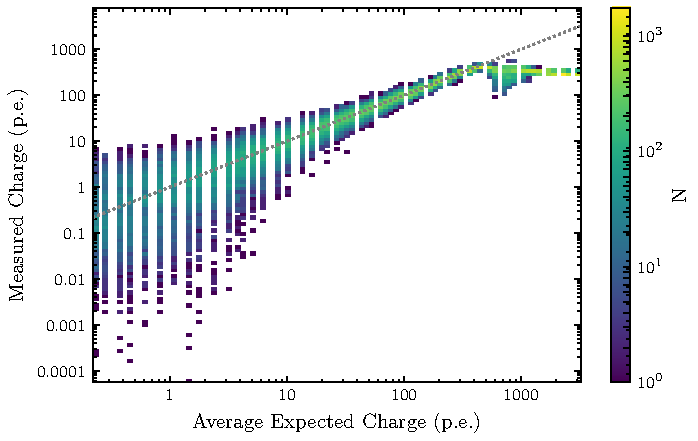
\includegraphics[width=\textwidth]{checs_mve_hist} 
	\caption[CHEC-S measured charge versus average expected charge.]{Two-dimensional histogram showing every measured charge for a single CHEC-S pixel, covering the full dynamic range. This dataset matches the one described in the \textit{Lab} procedure in Section~\ref{section:crprocedure}. The grey dotted line represents a one-to-one relation between the axes.}
	\label{fig:checs_mve_hist}
\end{figure}

\begin{figure}
	\centering
    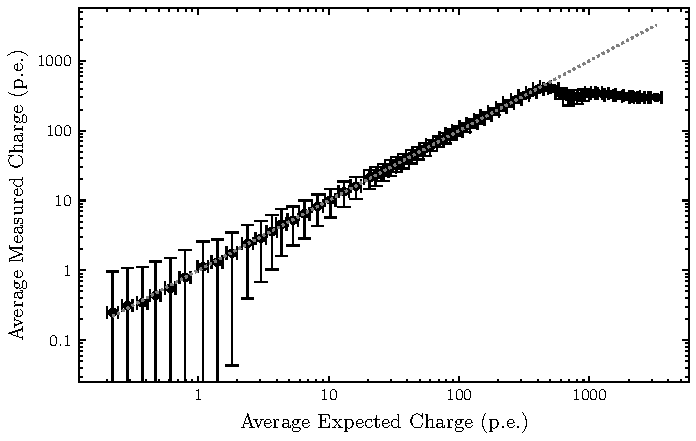
\includegraphics[width=\textwidth]{checs_mve_scatter} 
	\caption[CHEC-S average measured charge versus average expected charge.]{Similar to Figure~\ref{fig:checs_mve_hist}, but summarising the entries in terms of their averages and standard deviation for each illumination. The X error bars represent the uncertainty in the filter-wheel calibration into units of \si{\pe} (Section~\ref{section:fwerr}).}
	\label{fig:checs_mve_scatter}
\end{figure}

\begin{figure}
	\centering
    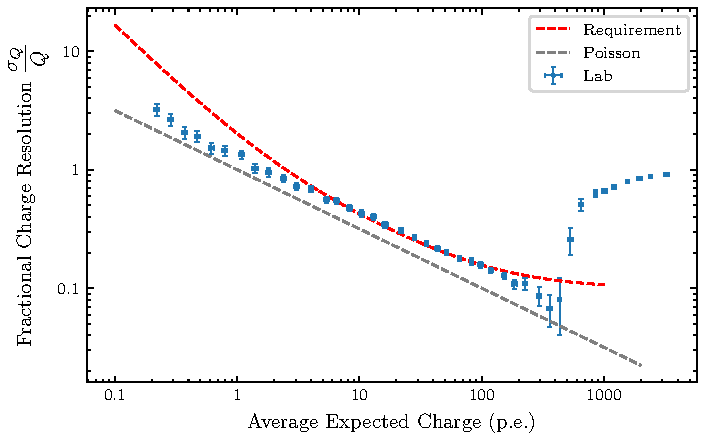
\includegraphics[width=0.9\textwidth]{cr_1_lab_raw} 
	\caption[\textit{Charge Resolution} of the Lab dataset in default units.]{\textit{Charge Resolution} for a single CHEC-S of the same Lab dynamic range dataset shown in Figure~\ref{fig:checs_mve_hist}. The Y error bars represent the standard deviation of the \textit{Charge Resolution} values across the camera. The X error bars represent the uncertainty in the filter-wheel calibration into units of \si{\pe} (Section~\ref{section:fwerr}). The presentation of the \textit{Charge Resolution} in this form matches Figure~\ref{fig:charge_res_req}.}
	\label{fig:cr_1_lab_raw}
\end{figure}

\begin{figure}
	\centering
    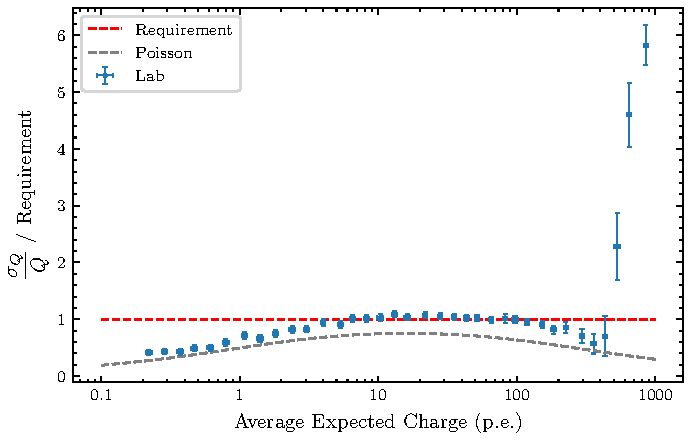
\includegraphics[width=0.9\textwidth]{cr_1_lab} 
	\caption[\textit{Charge Resolution} of the Lab dataset with respect to the requirement.]{Same as Figure~\ref{fig:cr_1_lab_raw}, but with respect to the requirement curve to emphasise the separation between it and the points.}
	\label{fig:cr_1_lab}
\end{figure}

To begin, the different representation of the \textit{Charge Resolution} are first explained in terms of the \textit{Lab} procedure and dataset. Figure~\ref{fig:checs_mve_hist} demonstrates the charge extracted for the entire dynamic range dataset, post calibration. It is the purpose of the \textit{Charge Resolution} to characterise the spread and bias of these measured charges from the average expected charge into a single value per average expected charge (or ``true charge'' where appropriate). The average measured charges in Figure~\ref{fig:checs_mve_scatter} seem to strongly follow a one-to-one relation with the average expected charge (in the non-saturated region), attesting to the success of the extracted charge calibration. However, to fully explore the performance of the camera, we continue on to the \textit{Charge Resolution} shown in Figure~\ref{fig:cr_1_lab_raw}. It is immediately obvious that in the saturated region (\SI{>300}{\pe}), the camera fails the \textit{Charge Resolution} requirement. This is expected, as we make no attempt to recover saturated signal in this investigation. Methods to account for the saturation are briefly described in Section~\ref{section:saturation}, and will be fully explored in a future investigation. To investigate other less obvious features in the \textit{Charge Resolution}, I display the \textit{Charge Resolution} in terms of its deviation from the requirement curve.

Figure~\ref{fig:cr_1_lab} shows the \textit{Charge Resolution} from Figure~\ref{fig:cr_1_lab_raw} divided by the requirement curve. This is how the \textit{Charge Resolution} is visualised elsewhere in this thesis, as it shows how close the points are to the requirement, and emphasises features that cause the results to fail the requirement. In the region of $10 < Q_\text{Exp} < 100$~\si{\pe}, the \textit{Charge Resolution} of the \textit{Lab} dataset fails requirements. By comparing this \textit{Charge Resolution} to those resulting from different Monte Carlo simulations that explore the contributing parameter space, we are able to identify the primary factors resulting in a failure to meet the requirement.

\subsection{Lab versus Monte Carlo}

\begin{figure}[H]
	\centering
    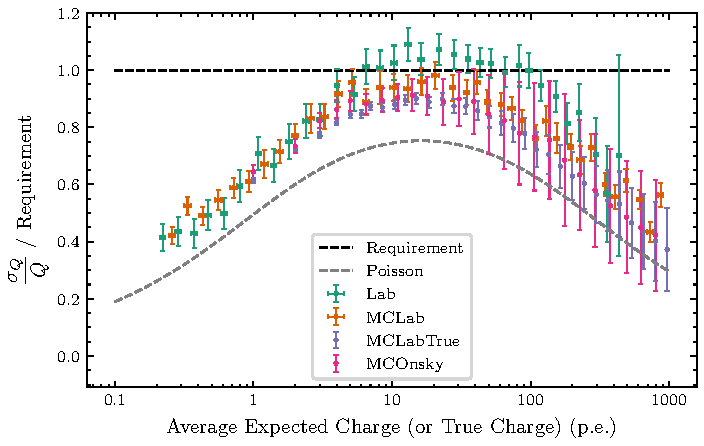
\includegraphics[width=\textwidth]{cr_2_lab_vs_mc} 
	\caption[Comparison of the different \textit{Charge Resolution} procedures.]{Comparison of the \textit{Charge Resolutions} resulting from the different procedures described in Section~\ref{section:crprocedure}. A background photon rate of \SI{5}{MHz} is simulated in the Monte Carlo datasets to represent the \gls{dcr} we expect inside the datasets produced from lab measurements.}
	\label{fig:cr_2_lab_vs_mc}
\end{figure}

As a preface to the simulated \textit{Charge Resolution} investigations, the differences in the procedures described in Section~\ref{section:crprocedure} are illustrated in Figure~\ref{fig:cr_2_lab_vs_mc}. The earlier descriptions of each procedure indicate the following expected differences between their \textit{Charge Resolutions}:
\begin{itemize}
\item With a perfect Monte Carlo model of the camera, there should be no differences between the \textit{Charge Resolution} of \textit{Lab} and \textit{MCLab}. Any deviations arise from a misunderstanding in the camera's behaviour, or from an unaccounted noise contribution.
\item The difference between \textit{MCLab} and \textit{MCLabTrue} demonstrates the expected change when transitioning from the average expected charge, to the ``true charge'' that was detected in the pixel.
\item As they are the same camera model, and the same \textit{Charge Resolution} calculation approach, there should be very little difference between \textit{MCLabTrue} and \textit{MCOnsky}. The only factor to contribute to differences between the two procedures is the peak-finding that is necessary for the \textit{MCOnsky} datasets.
\end{itemize}

It is therefore apparent in Figure~\ref{fig:cr_2_lab_vs_mc} that our simulation model is not a perfect representation of \gls{chec-s}. The lack of saturation in the simulated datasets is expected, and that is a feature we will include in future investigations. However, from the simulated datasets we can conclude that in the absence of additional \gls{nsb} photons, the \textit{Charge Resolution} of our camera before the saturated region should be below the requirement. As we do not observe this in the non-simulated dataset, there must be a noise contribution we have not appropriately accounted for. The work required to fully diagnose this noise contribution is beyond the scope of this thesis, however possible options include:
\begin{description}
\item [Transfer Functions] The simulations do not fully simulate the \gls{chec-s} electronics. They contain no resemblance of the digitising behaviour of \gls{target} \glspl{asic}, and therefore no variations in amplitude response exists from sample-to-sample. Inaccuracies in the Transfer Function calibration (Chapter~\ref{ch5-calibration}) could manifest themselves as differences between the \textit{Charge Resolutions} of lab and simulated data.
\item [Timing] As mentioned in Section~\ref{section:timing_corrections}, the variations in signal arrival time between pixels could degrade the \textit{Charge Resolution}. This contribution is not included in the simulation.
\item [Electrical Crosstalk] Inside the simulation, each pixel is considered independently. Due to electronic coupling, this is unfortunately not the case in reality. \change{Rich: better description (technical) of how the electronic crosstalk happens, e.g. of ground bounce}
\item [Optical Crosstalk] Although the optical crosstalk is included into the simulation via the \gls{spe} spectrum shape, this may not fully characterise the behaviour of the optical crosstalk. \change{Rich: HOW?}
\item [Reference Pulse Shape] Another major difference between simulation and reality is the behaviour of the pulse shape. In simulations, the pulse shape at all illuminations is constructed by the superposition of the individual photoelectron pulses. If that description was appropriate for the real camera, the pulse shape dependency with amplitude would not be seen in Section~\ref{section:pulse_shape_results}. As we use the \textit{Cross Correlation} charge extraction method, the measured charge is sensitive to changes in pulse shape. This could, in theory, result in discrepancies between the \textit{Charge Resolutions} of lab and simulated data. However, the investigations in Appendix~\ref{a3-extractors} seem to suggest this factor is not significant.
\end{description}

Identifying the cause of this noise contribution is of paramount importance in the commissioning of \gls{chec-s}. However, the remainder of this section will explore the possibility of meeting the \textit{Charge Resolution} even in the presence of this unknown noise contribution. This procedure may give insight into the source of the noise.

\subsection{Night Sky Background}

\begin{figure}[H]
	\centering
    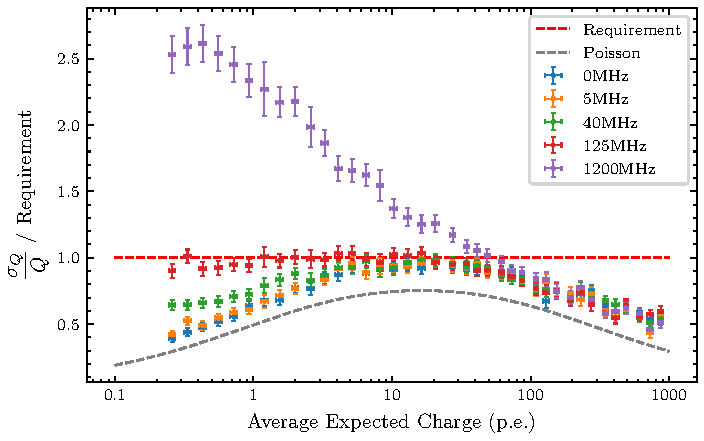
\includegraphics[width=\textwidth]{cr_3_nsb_comparison_mclab} 
	\caption[Comparison of the \textit{Charge Resolution} at different NSBs.]{Comparison of the \textit{Charge Resolutions} obtained from the \textit{MCLab} procedure when simulating different values of Night Sky Background (NSB).}
	\label{fig:cr_3_nsb_comparison_mclab}
\end{figure}

At higher values of \gls{nsb}, we expect higher amounts of noise to be included in the charge extraction, resulting in a higher charge then expected, and increasing the variation in signal measured for the same average illumination. Figure~\ref{fig:cr_3_nsb_comparison_mclab} illustrates the degradation in charge resolution caused by an increase in \gls{nsb} rate. The effects are most pronounced at the lower values of average expected charge, where an increase in \gls{nsb} has a larger impact on the signal-to-noise ratio. We can conclude from this figure that even if the unknown noise contribution in the \textit{Lab} datasets is corrected for, the current design of \gls{chec-s} could potentially fail to meet the \gls{cta} requirement at the specified \gls{nsb} of \SI{125}{MHz}.

\begin{figure}
	\centering
    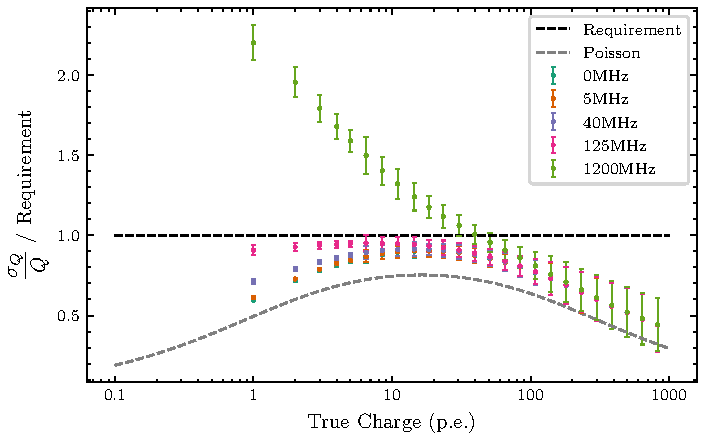
\includegraphics[width=\textwidth]{cr_3_nsb_comparison_mclabtrue} 
	\caption[Comparison of the \textit{Charge Resolution} at different NSBs using the \textit{MCLabTrue} procedure.]{Comparison of the \textit{Charge Resolutions} obtained from the \textit{MCLabTrue} procedure when simulating different values of NSB.}
	\label{fig:cr_3_nsb_comparison_mclabtrue}
\end{figure}

A similar dependence on \gls{nsb} is observed with the \textit{MCLabTrue} procedure in Figure~\ref{fig:cr_3_nsb_comparison_mclabtrue}, however the \textit{Charge Resolutions} demonstrate an overall improved performance over the \textit{MCLab} representation.

\begin{figure}
	\centering
    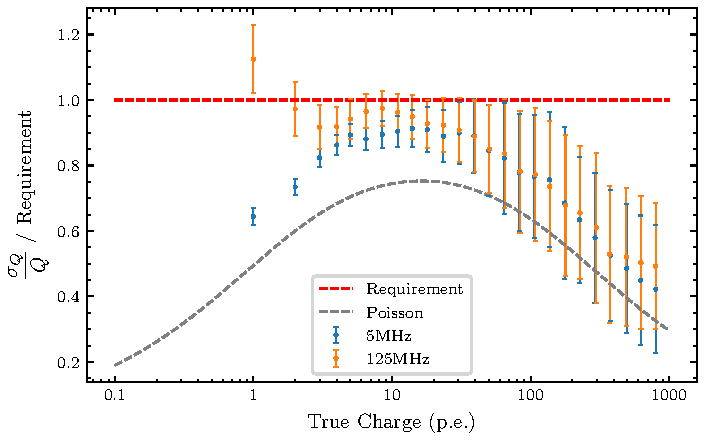
\includegraphics[width=\textwidth]{cr_3_nsb_comparison_mconsky} 
	\caption[Comparison of the \textit{Charge Resolution} at two different NSBs when observing Cherenkov showers (via the\textit{MCOnsky} procedure).]{Comparison of the \textit{Charge Resolutions} obtained from simulated observations of Cherenkov showers (via the \textit{MCOnsky} procedure), when simulating different values of NSB. The signal inside each waveform is found with the \textit{Local Peak Finding} approach.}
	\label{fig:cr_3_nsb_comparison_mconsky}
\end{figure}

Despite the improved performance achieved when using the ``true charge'', a second consequence of higher \gls{nsb} is the increased difficulty of finding the signal pulse among the noise pulses. As shown in Figure~\ref{fig:cr_3_nsb_comparison_mconsky}, this causes the current model of \gls{chec-s} to fail the \textit{Charge Resolution} requirement when observing Cherenkov showers. An alternative to the \textit{Local Peak Finding} approach could improve on this bias to noise pulses, and therefore allow the requirement to be met.

\subsection{Optical Crosstalk}

\begin{figure}[H]
	\centering
    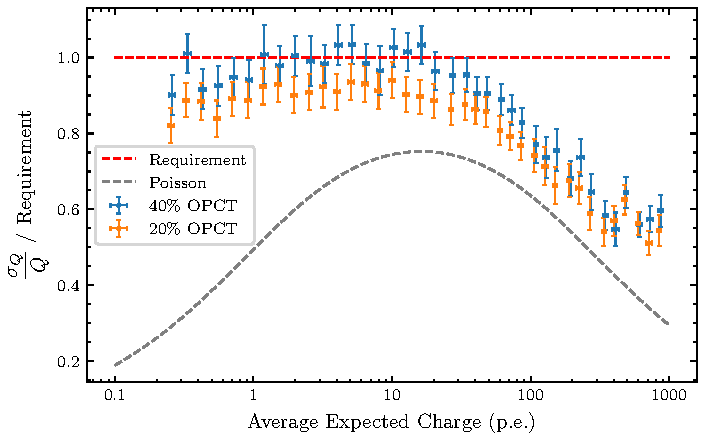
\includegraphics[width=\textwidth]{cr_4_opct_mc} 
	\caption[Comparison of the \textit{Charge Resolution} at different values of optical crosstalk.]{Comparison of the \textit{Charge Resolutions} obtained from the \textit{MCLab} procedure when simulating different values of optical crosstalk. An \gls{nsb} rate of \SI{125}{MHz} was included in these simulations.}
	\label{fig:cr_4_opct_mc}
\end{figure}

A prime suspect for the poor \textit{Charge Resolution} is the very high (\SIrange{35}{40}{\percent}) optical crosstalk in the \glspl{sipmt} currently used for the \gls{chec-s} prototype. The optical crosstalk contributes to the extracted charge in two ways: 
\begin{itemize}
\item The measured charge is consistently higher. This factor is accounted for in the flat-fielding calibration.
\item The spread in charge that results from a particular amount of photons contains a higher variation. This is therefore expressed as an increase in the Excess Noise Factor (ENF).
\end{itemize}

\subsubsection{Monte Carlo}

Figure~\ref{fig:cr_4_opct_mc} demonstrates the \textit{MCLab Charge Resolution} for a simulation of the \gls{chec-s} model, but with \SI{20}{\percent} optical crosstalk. The effect of a reduced optical crosstalk is a consistent improvement in the \textit{Charge Resolution} for all illuminations.

\begin{figure}[H]
	\centering
    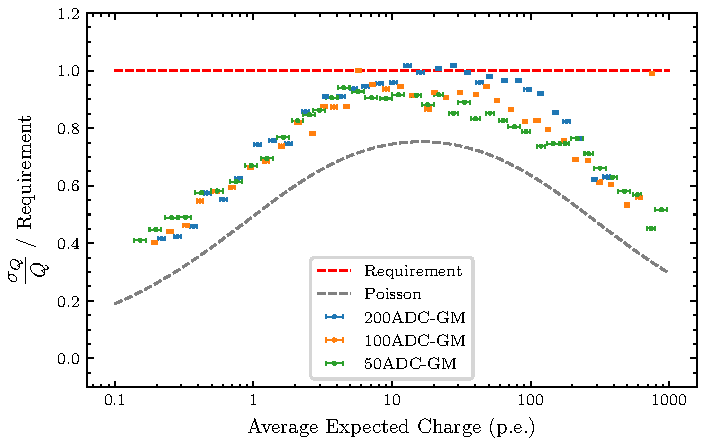
\includegraphics[width=\textwidth]{cr_4_opct_biasvoltage} 
	\caption[Comparison of the \textit{Lab Charge Resolution} with different bias voltages applied to the \gls{sipmt} pixel.]{Comparison of the \textit{Charge Resolutions} obtained from different \textit{Lab} datasets, each dataset gain matched to a different ADC value. By gain matching to different ADC values, a different bias voltage is applied to the \gls{sipmt} pixel. As this dataset was gain matched in units of ADC, the spread between pixels is large, and is therefore excluded from this figure to guarantee the effects on a single pixel are visible.}
	\label{fig:cr_4_opct_biasvoltage}
\end{figure}

\subsubsection{Changing Bias Voltage}

Due to the dependence of the optical crosstalk on the bias voltage across the \gls{sipmt} \change{check with rich on parameter dependencies}, we were able to investigate the impact a reduced optical crosstalk has on \textit{Charge Resolution} with \textit{Lab} data. Three datasets were generated, each gain matched to a different ADC value (the transfer function were not included in the gain matching procedure at the time). A lower bias voltage is required to obtain a smaller gain-matched setting. Figure~\ref{fig:cr_4_opct_biasvoltage} shows the improvement in \textit{Charge Resolution} with reduced bias voltage, bringing the result lower than the requirement. The effect is not identical to what is observed in simulations of a lower optical crosstalk, but the lower bias results do seem to correct for the region where the unknown additional noise component is apparent. Further investigation into this behaviour is required.

However, it is important to note that the reduction in bias voltage also results in a decrease of Photon Detection Efficiency (PDE). The effect of a lower PDE is a reduction in the camera's ability to resolve Cherenkov shower photons. This contradiction between improving \textit{Charge Resolution}, but reducing Cherenkov shower resolution, is one of the primary reasons the \gls{cta} requirements are being redefined to be in terms of photons, as described in Chapter~\ref{ch3-architecture}.

\subsection{Conclusion}

As suggested by the investigations in this sections, a reduction in optical crosstalk could allow \gls{chec-s} to meet the \textit{Charge Resolution} requirement for all calculation procedures. 

\notes{Need to reduce opct without reducing bias voltage - better detectors}

\notes[inline,caption={}]{
	\begin{itemize}
		\item Can we meet requirement with lower opct? Describe opct to ENF, Fit lab data with equation, show with enf equation at 125 MHz
	\end{itemize}
}

\section{CHEC-S Pulse Shape} \label{section:pulse_shape_results}

\section{CHEC-S Time Resolution}

\section{CHEC-M}

\notes[inline]{Comparison in performance between CHEC-M and CHEC-S. show SPE spectrum again, huge decrease in spe\_sigma}



